% K-Full-MPC is the whole outer-loop controller (no LQR).
% Build: see presentation/diagrams/README.md.
\documentclass[tikz, border=4pt]{standalone}
% Shared style for the slide block diagrams. Colours match report/koopman_mpc.tex.
\usepackage{amsmath,amssymb}
% Lato matches the slides; plain TeX Live may not ship it, so fall back to the default sans.
\IfFileExists{lato.sty}{\usepackage[default]{lato}}{\renewcommand{\familydefault}{\sfdefault}}
\usepackage{tikz}
\usetikzlibrary{positioning, arrows.meta, fit, calc}

\definecolor{boxfill}{HTML}{EAF2FB}
\definecolor{boxdraw}{HTML}{3B6EA8}
\definecolor{hlfill}{HTML}{FDE6D8}
\definecolor{hldraw}{HTML}{D9622B}
\definecolor{subtxt}{HTML}{555555}
\definecolor{plantdraw}{HTML}{6B6B6B}
\definecolor{windfill}{HTML}{E6F4EA}
\definecolor{winddraw}{HTML}{3C8D5A}
\definecolor{mpcfill}{HTML}{F6E6F0}
\definecolor{mpcdraw}{HTML}{A8507F}

\tikzset{
  block/.style = {draw=boxdraw, fill=boxfill, rounded corners=3pt,
    line width=0.7pt, align=center, minimum height=13mm, inner xsep=6pt},
  hl/.style    = {block, draw=hldraw, fill=hlfill},
  mpc/.style   = {block, draw=mpcdraw, fill=mpcfill, line width=1.1pt},
  windb/.style = {block, draw=winddraw, fill=windfill, minimum height=10mm},
  plant/.style = {draw=plantdraw, dashed, rounded corners=5pt,
    line width=0.8pt, inner xsep=4mm, inner ysep=4mm},
  sum/.style   = {draw=boxdraw, fill=white, circle, line width=0.7pt,
    minimum size=6mm, inner sep=0pt},
  sig/.style   = {-{Stealth[length=2.4mm]}, line width=0.7pt},
  fb/.style    = {sig, draw=subtxt},
  dot/.style   = {circle, fill=black, inner sep=1.3pt},
  lab/.style   = {above, font=\small, inner sep=3pt},
}
% Second line of a block in grey, smaller.
\newcommand{\sub}[1]{\\[-1pt]{\footnotesize\color{subtxt}#1}}

\begin{document}
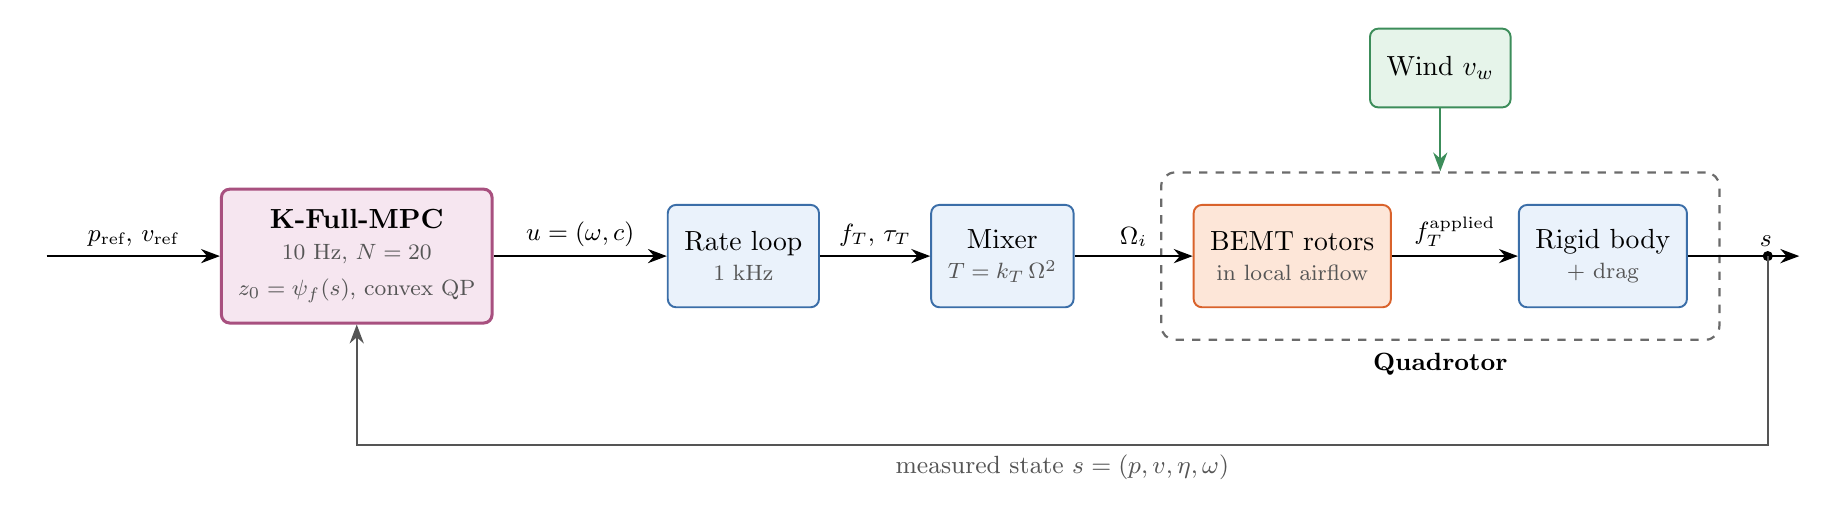
\begin{tikzpicture}[node distance=9mm]
  \node (ref) {};
  \node[mpc, right=22mm of ref, minimum height=17mm] (kfull)
    {\textbf{K-Full-MPC}\sub{10 Hz, $N = 20$}\\[1pt]
     {\footnotesize\color{subtxt}$z_0 = \psi_f(s)$, convex QP}};
  \node[block, right=22mm of kfull] (rate) {Rate loop\sub{1 kHz}};
  \node[block, right=14mm of rate]  (mix)  {Mixer\sub{$T = k_T\,\Omega^2$}};
  \node[hl,    right=15mm of mix]   (bemt) {BEMT rotors\sub{in local airflow}};
  \node[block, right=16mm of bemt]  (body) {Rigid body\sub{+ drag}};
  \node[plant, fit=(bemt)(body)]    (plantbox) {};
  \node[below=1pt of plantbox.south, font=\small\bfseries] {Quadrotor};
  \node[windb, above=8mm of plantbox] (wind) {Wind $v_w$};
  \coordinate[right=10mm of plantbox.east] (out);

  \draw[sig] (ref) -- node[lab] {$p_\text{ref},\,v_\text{ref}$} (kfull);
  \draw[sig] (kfull) -- node[lab] {$u = (\omega, c)$} (rate);
  \draw[sig] (rate) -- node[lab] {$f_T,\,\tau_T$} (mix);
  \draw[sig] (mix)  -- node[lab] {$\Omega_i$} (bemt);
  \draw[sig] (bemt) -- node[lab] {$f_T^{\text{applied}}$} (body);
  \draw[sig] (body) -- node[lab, pos=0.7] {$s$} (out);
  \draw[sig, draw=winddraw] (wind) -- (plantbox);

  % State feedback
  \coordinate (fbx) at ($(out) + (-4mm, 0)$);
  \node[dot] at (fbx) {};
  \draw[fb] (fbx) -- ++(0, -24mm) -| (kfull.south)
    node[pos=0.25, below, font=\small, text=subtxt] {measured state $s = (p, v, \eta, \omega)$};
\end{tikzpicture}
\end{document}
